\documentclass{prova}

\usepackage{amssymb}
\usepackage{amsmath}

\setlength{\topmargin}{-2.5cm}
\setlength{\textheight}{26cm}

\professor{Prof.\@ Adriano Barbosa}
\disciplina{N\'umeros e Fun\c{c}\~oes Reais}
\avaliacao{1}
\curso{PROFMAT}
\data{20/05/2022}

\begin{document}
	\cabecalho{5}  % o numero 5 indica a qnt de quadros na tabela de nota
    \vspace{-0.6cm}
	\begin{questionario}
        \q{Sejam $X_1$, $X_2$, $Y_1$, $Y_2$ subconjuntos do conjunto universo
            $U$. Suponha que $X_1\cup X_2=U$ e $Y_1\cap Y_2=\varnothing$, que
            $X_1\subset Y_1$ e que $X_2\subset Y_2$. Prove que $X_1=Y_1$ e
            $X_2=Y_2$.}
        \q{Considere as seguintes (aparentes) equival\^encias l\'ogicas:}
            \begin{align*}
                x=1 &\Leftrightarrow x^2-2x+1=0 \\
                    &\Leftrightarrow x^2-2\cdot 1+1=0 \\
                    &\Leftrightarrow x^2-1=0 \\
                    &\Leftrightarrow x=1 \text{ ou } x=-1
            \end{align*}
            Conclus\~ao: $x=1 \Leftrightarrow x=\pm 1$. Onde est\'a o erro?
        \q{Use indu\c{c}\~ao para provar que
        $1^3+2^3+3^3+\cdots+n^3=\displaystyle\frac{1}{4}n^2(n+1)^2$.}
        \q{Seja $X\subset\mathbb{N}$ um conjunto n\~ao-vazio com a seguinte
            propriedade: para qualquer $n\in\mathbb{N}$, se todos os n\'umeros
            naturais menores do que $n$ pertencem a $X$ ent\~ao $n\in X$. Prove que
            $X=\mathbb{N}$. (Sugest\~ao: boa ordena\c{c}\~ao)}
        \q{Prove, por indu\c{c}\~ao, que um conjunto com $n$ elementos possui $2^n$
            subconjuntos.}
        \q{Verifique se cada passo na solu\c{c}\~ao das inequa\c{c}\~oes abaixo est\'a
            correto:}
            \begin{questionario}
                \qq{$\displaystyle\frac{5x+3}{2x+1}>2 \Rightarrow 5x+3>4x+2
                    \Rightarrow x>-1$}
                \qq{$\displaystyle\frac{2x^2+x}{x^2+1}<2 \Rightarrow
                    2x^2+x<2x^2+2 \Rightarrow x<2$}
            \end{questionario}
        \q{Considere todos os intervalos da forma $[0,\frac{1}{n}]$, onde
            $n\in\mathbb{N}$. Existe um n\'umero comum a todos estes intervalos? E se
            forem tomados os intervalos abertos?}
        \q{Um garoto brinca de arrumar palitos fazendo uma sequ\^encia de
            hex\'agonos como na figura. Se ele fez 2022 hex\'agonos, quantos palitos
            utilizou?}
            \begin{figure}[h]
                \centering
                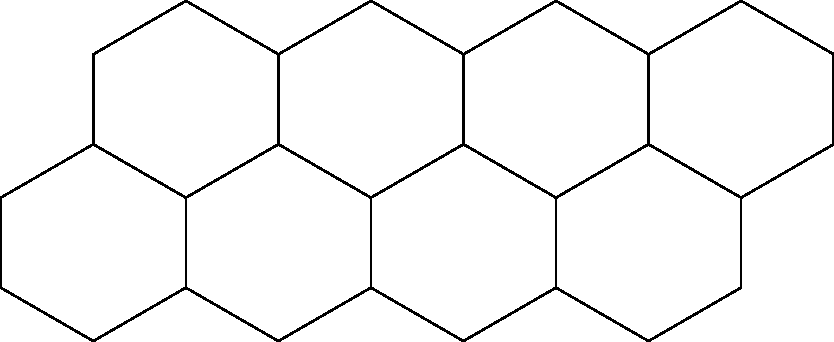
\includegraphics[width=0.5\textwidth]{fig1.pdf}
            \end{figure}
    \end{questionario}
\end{document}
